\begin{figure}[h]
  \centering
  \scalebox{0.65}{
    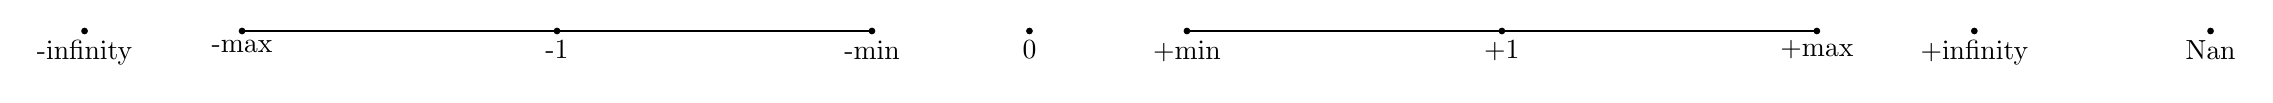
\begin{tikzpicture}
      \filldraw (0,0) circle (1pt) node[align=center, below] {-infinity};
      \filldraw (2,0) circle (1pt) node[align=center, below] {-max};
      \filldraw (6,0) circle (1pt) node[align=center, below] {-1};
      \filldraw (10,0) circle (1pt) node[align=center, below] {-min};
      \filldraw (12,0) circle (1pt) node[align=center, below] {0};
      \filldraw (14,0) circle (1pt) node[align=center, below] {+min};
      \filldraw (18,0) circle (1pt) node[align=center, below] {+1};
      \filldraw (22,0) circle (1pt) node[align=center, below] {+max};
      \filldraw (24,0) circle (1pt) node[align=center, below] {+infinity};
      \filldraw (27,0) circle (1pt) node[align=center, below] {Nan};

      \draw[-](2,0) -- (10, 0);
      \draw[-](14,0) -- (22, 0);

    \end{tikzpicture}
  }
  \caption{\label{float_point_size} Range of representable values with floating point types}
\end{figure}
